
\chapter{Running the model: a practice simulation}

\label{loc:contact1}

This chapter is meant for first-time users of the LMD model.
As the best introduction to the model is surely to run a simulation,
here we explain how to go about it.
All you will need are files necessary to build the GCM (all are in
the {\tt LMDZ.GENERIC} directory) as well as some initial states
to initiate simulations (see below).\\
Once you have followed the example given below,
you can then go on to change the control parameters and the initial states
as you wish. A more detailed description of the model's organization
as well as associated inputs and
outputs are given in sections~\ref{sc:info} and~\ref{sc:io}.

\section{Installing the model from SVN}

The first thing is to download the model from our SVN server. If you cannot use SVN, just find an old school way to get a copy of the basic model directory \verb"LMDZ.GENERIC" (and all the other source files needed for visualization) and download it to your account. Then start directly from the fifth point.

\begin{description}
\item[$\bullet$] Go to the directory where you want to download the model. Not that only one directory (the root directory) will be added in the current directory.

\item[$\bullet$] If svn is installed on your system, set up the root directory by tipping 
\begin{verbatim}
svn co "http://svn.lmd.jussieu.fr/Planeto/trunk" -N Name_of_root_directory
cd Name_of_root_directory
\end{verbatim}

\item[$\bullet$] You can now download one of the LMDZ models (for Generic, Mars, Venus, Titan, ...) by tipping
\begin{verbatim}
svn update LMDZ.MODEL_YOU_WANT
\end{verbatim}
For the Generic model, just tipe
\begin{verbatim}
svn update LMDZ.GENERIC
\end{verbatim}
The contents of the directory that has been created are described in Chapter \ref{loc:contenu}.

\item[$\bullet$] For visualization of the simulations, yo will need some utilities that we might as well download now by doing
\begin{verbatim}
svn update UTIL
\end{verbatim}

\item[$\bullet$] Now we must set up the {\tt makegcm} script that will perform the compilation of the model. Go into the {\tt LMDZ.GENERIC} directory and edit the appropriate \verb"makegcm_mycompiler" (hereafter called \verb"makegcm"), where \verb"mycompiler" is the compiler that you want to use.
There are two important environment variables concerning source files that are initialized by \verb"makegcm" and that we need to set properly:
\begin{enumerate}
\item \verb"LMDGCM", the path to the source files. By default, the line
\begin{verbatim}
setenv LMDGCM `readlink -f $scriptdir`
\end{verbatim}
allows \verb"makegcm" to assume that it is executed in the root source directory so that this should work without any change. If \verb"makegcm" does not find the source, you can enter manually the path by changing the above line by
 \begin{verbatim}
setenv LMDGCM "path/to/source/directory/LMDZ.GENERIC"
\end{verbatim}
\item \verb"LIBOGCM", the path to the compilation directory where all object files will be kept. By default, the line
\begin{verbatim}
setenv LIBOGCM $LMDGCM/libo
\end{verbatim}
specifies that source will be kept in a \verb"libo" directory created in \verb"LMDZ.GENERIC". You can also change that if needed.
\end{enumerate} 

\item[$\bullet$]Install NetCDF
%\item {\bf -} \htmladdnormallink{Install NetCDF}
{http://www.unidata.ucar.edu/packages/netcdf/INSTALL.html}
and set environment variables  \verb"NCDFINC" and \verb"NCDFLIB":

  \begin{description}
  \item The latest version of the NetCDF package is available on the web at the following address: {http://www.unidata.ucar.edu/software/netcdf}
  along with instructions for building (or downloading precompiled
  binaries of) the library.
  \item Once the NetCDF library has been compiled (or downloaded),
  you should have access to the library {\tt libnetcdf.a} itself,
  the various files ({\tt netcdf.inc}, {\tt netcdf.mod}, ...)
  to include in programs, and basic NetCDF software ({\it ncdump}
  and {\it ncgen}).

  \item To ensure that during compilation, the model can find the
  NetCDF library and include files,
  you must declare environment variables \verb"NCDFLIB" and \verb"NCDFINC".

  \item \verb"NCDFLIB" must contain the path to the directory containing
   the object library {\tt libnetcdf.a}
   and \verb"NCDFINC" must contain the path to the directory containing
   the include files ({\tt netcdf.inc},...)\\
As for \verb"LMDGCM" variable, these variables can be declared by changing the right line in \verb"makegcm"
  \begin{verbatim}
  setenv NCDFINC /wherever/is/netcdf/include
  setenv NCDFLIB /wherever/is/netcdf/lib
  \end{verbatim}
For example, if working at LMD and with \verb"ifort", the path is  
   \begin{verbatim}
  setenv NCDFINC /donnees/emlmd/netcdf64-4.0.1_ifort/include
  setenv NCDFLIB /donnees/emlmd/netcdf64-4.0.1_ifort/lib
  \end{verbatim}
  \end{description}
  
\item[$\bullet$] Install software for loading and displaying NetCDF files
   such as GrAdS (http://grads.iges.org/grads/), Ferret (http://ferret.wrc.noaa.gov/Ferret), or Python. Some visualization scripts, especially for Python, can be found in the 
\verb"UTIL" directory and will be described later.


\item[$\bullet$] Finally, make sure that you have access to all the executables
needed for building and using the model and
remember to set environment variables to the correct corresponding pathes
(note that if you do not want to have to redefine these every session,
you should put the definitions in the corresponding {\tt .cshrc} or
{\tt .bashrc} files).

  \begin{description}
  \item {\bf -} UNIX function {\it make}
  \item {\bf -} a Fortran compiler
  \item {\bf -} ncdump
  \item {\bf -} grads (or ferret)
  \end{description}

\end{description}


\section{Installing the model without SVN}

 Create an alias so that the compilation script {\bf makegcm}
  is available from anywhere (more convinient than having to type the full
  path to the script, or copying it over where you want to run it).
  The {\tt makegcm} script is in the LMDZ.GENERIC directory, which
  is referenced by the {\bf LMDGCM} variable, so:\\
  If using Csh:
  \begin{verbatim}
  alias makegcm $LMDGCM'/makegcm'
  \end{verbatim}
  if using Bash:
  \begin{verbatim}
  alias makegcm=$LMDGCM/makegcm
  \end{verbatim}

\section{Compiling the LMDZ.GENERIC model (sequential only)}
\label{sc:run1}

Two options exist to compile the model. 
\begin{enumerate}
\item Create an alias so that the compilation script \verb"makegcm"
  is available from anywhere.
  If using Csh:
  \begin{verbatim}
  alias makegcm 'path/to/LMDZ.GENERIC/makegcm'
  \end{verbatim}
  if using Bash:
  \begin{verbatim}
  alias makegcm=path/to/LMDZ.GENERIC/makegcm
  \end{verbatim}
Then the compilation is done by tipping 
  \begin{verbatim}
makegcm -options gcm
  \end{verbatim}
This solution can be convenient but is less flexible if you want to compile the model in many different configurations and keep track of it.

\item Create and edit an executable script (that we will call \verb"compile") in the directory where you will want to run the model. Put the line
  \begin{verbatim}
/path/to/the/model/I/use/makegcm -options gcm
  \end{verbatim}
The advantage of this option is that the \verb"compile" is present in all of the working directories where the model is ran, allowing you to keep track of the options used.
\end{enumerate}

Just remains to choose the options. The basic options are as follows
\begin{verbatim}
makegcm -d LONxLATxALT -p std -t XX -s YY -b IRxVI gcm
\end{verbatim}
where \verb"LONxLATxALT" are the number of grid cells in longitude, latitude and altitude, \verb"XX" is the number of tracers, \verb"YY" is the number of scatterers that will be taken into account in the radiative code and \verb"IRxVI" is the number of spectral bands in the thermal emission and stellar part of the radiative code. The option \verb"-debug" is available with most compilers. The code runs much more slowly but can output more user friendly bug report messages.

{\bf -} Example 1: Compiling the generic model at grid resolution 64x48x20
for example, type (in compliance with the manual for the makegcm function
given in section~\ref{sc:compil1})

\begin{verbatim}
makegcm -d 64x48x20 -p std gcm
\end{verbatim}

\noindent
You can find executable {\bf gcm.e} (the compiled model) in the directory
where you ran the makegcm command.

{\bf -} Example 2: Compiling the generic model with 2 tracers
(e.g. water vapour and ice to simulate the water cycle):
\begin{verbatim}
makegcm -d 32x32x20 -t 2 -p std gcm
\end{verbatim}

{\bf -} Example 3:
Compiling the the generic model to check for and trace errors (with ifort compiler -
useful for debugging - warning, the model then runs very slowly!):
\begin{verbatim}
makegcm -d 32x32x20 -p std -O "-g -fpe0 -traceback" gcm
\end{verbatim}
%**********
\section{Compiling the LMDZ.COMMON model (sequential or parallel)}
\label{sc:run1_common}
\begin{enumerate}
\item Prerequisites:
\begin{itemize}
\item[$\bullet$] Downloaded LMDZ.COMMON and LMDZ.OTHER\_MODEL containing the physic you want.
\item[$\bullet$] Available MPI library and wrapped compiler (mpif90, mpiifort,...)
\item[$\bullet$] Optional (but recommended) fcm:
\begin{itemize}
\item LMD: /distrib/local/fcm/bin
\item Ciclad: /home/millour/FCM\_V1.2/bin
\item Gnome: /san/home/millour/FCM\_V1.2/bin
\item Other: fcm is just a collection of perl scripts; can be copied over on any other machine, or simply downloaded using svn:\\
svn checkout http://forge.ipsl.jussieu.fr/fcm/svn/PATCHED/FCM\_V1.2
\end{itemize}
\end{itemize}
\item Then choose the physic you want to couple with the LMDZ.COMMON dynamic core by creating a symbolic link in the LMDZ.COMMON/libf directory.\\
If you want to use mars physic:
\begin{verbatim}
cd LMDZ.COMMON/libf
ln -s path/to/LMDZ.MARS/libf/phymars .
ln -s path/to/LMDZ.MARS/libf/aeronomars .
\end{verbatim}
Here, we want the LMDZ.GENERIC physic phystd:
\begin{verbatim}
cd LMDZ.COMMON/libf
ln -s path/to/LMDZ.GENERIC/libf/phystd .
\end{verbatim}
\item  To compile in LMDZ.COMMON directory:
\begin{verbatim}
./makelmdz_fcm -s XX -t XX -d LONxLATxALT -b IRxVI -p physicSuffix 
-arch archFile [-parallel mpi/mpi_omp] gcm
\end{verbatim}
\begin{itemize}
\item[$\bullet$] \textbf{physicSuffix} is \verb|mars| for phymars, \verb|std| for phystd...
\item[$\bullet$] \textbf{archFile} is the name of configuration files from LMDZ.COMMON/arch: use \verb|CICLADifort| the ifort compiler in a CICLAD environment, \verb|X64_ADA| for the ADA architecture...
\item[$\bullet$] To compile in parallel with mpi, add \verb|-parallel mpi| option. By default it is serial code.
\item[$\bullet$] For hybrid MPI-OpenMP parallelisation, add \verb|-parallel mpi_omp| option.
\item[$\bullet$] For faster compilation, the option \verb|-j N| uses N simultaneous tasks.
\item[$\bullet$] \verb|-full| option forces full (re)-compilation from scratch.
\item[$\bullet$] Created program is in LMDZ.COMMON/bin directory, with dimensions included in the program name. e.g.: gcm\_64x48x29\_phymars\_para.e
\end{itemize}
\end{enumerate}
NB: It is possible to compile without fcm by replacing \verb|makelmdz_fcm| by \verb|makelmdz|. Created program is in LMDZ.COMMON directory and named gcm.e.
%**********
\section{Input files (initial states and def files)}
{\bf -} In directory \verb+LMDZ.GENERIC/deftank+
you will find some examples of run
parameter files ({\tt .def} files) which the model needs at runtime.
The four files the model requires (they must be in the same directory as the
executable {\tt gcm.e}) are:
{\bf run.def} (described in
section~\ref{loc:entrees}) {\bf callphys.def}
(see section~\ref{sc:callphys.def}),
{\bf gases.def}, {\bf z2sig.def} and {\bf traceur.def}.\\

The example {\tt .def} files given in the {\tt deftank} directory
are for various configurations (e.g. model resolution, planet type), copy (and eventually
rename these files to match the generic names) to the directory where
you will run the model.\\

\noindent
{\bf -} Copy initial condition files
{\bf start.nc} and {startfi.nc}  (described in section
\ref{loc:entrees}) to the same directory.\\
You can extract such files from {\bf start\_archive}
`banks of initial states' (i.e. files which
contain collections of initial states from
stndard scenarios and which can thus be used
to check if the model is installed correctly) stored on the LMD website at\\
\verb+http://www.lmd.jussieu.fr/~forget/datagcm/Starts+.
See section~\ref{sc:newstart} for a description of how to proceed to
extract {\bf start} files from {\bf start\_archives}.\\

[NOTE: WITH THE GENERIC MODEL WE ALMOST ALWAYS START FROM ``startplanet'' FILES]
%**********
\section{Running the model}
\begin{figure}
\centerline{\framebox[1.4\textwidth][c]{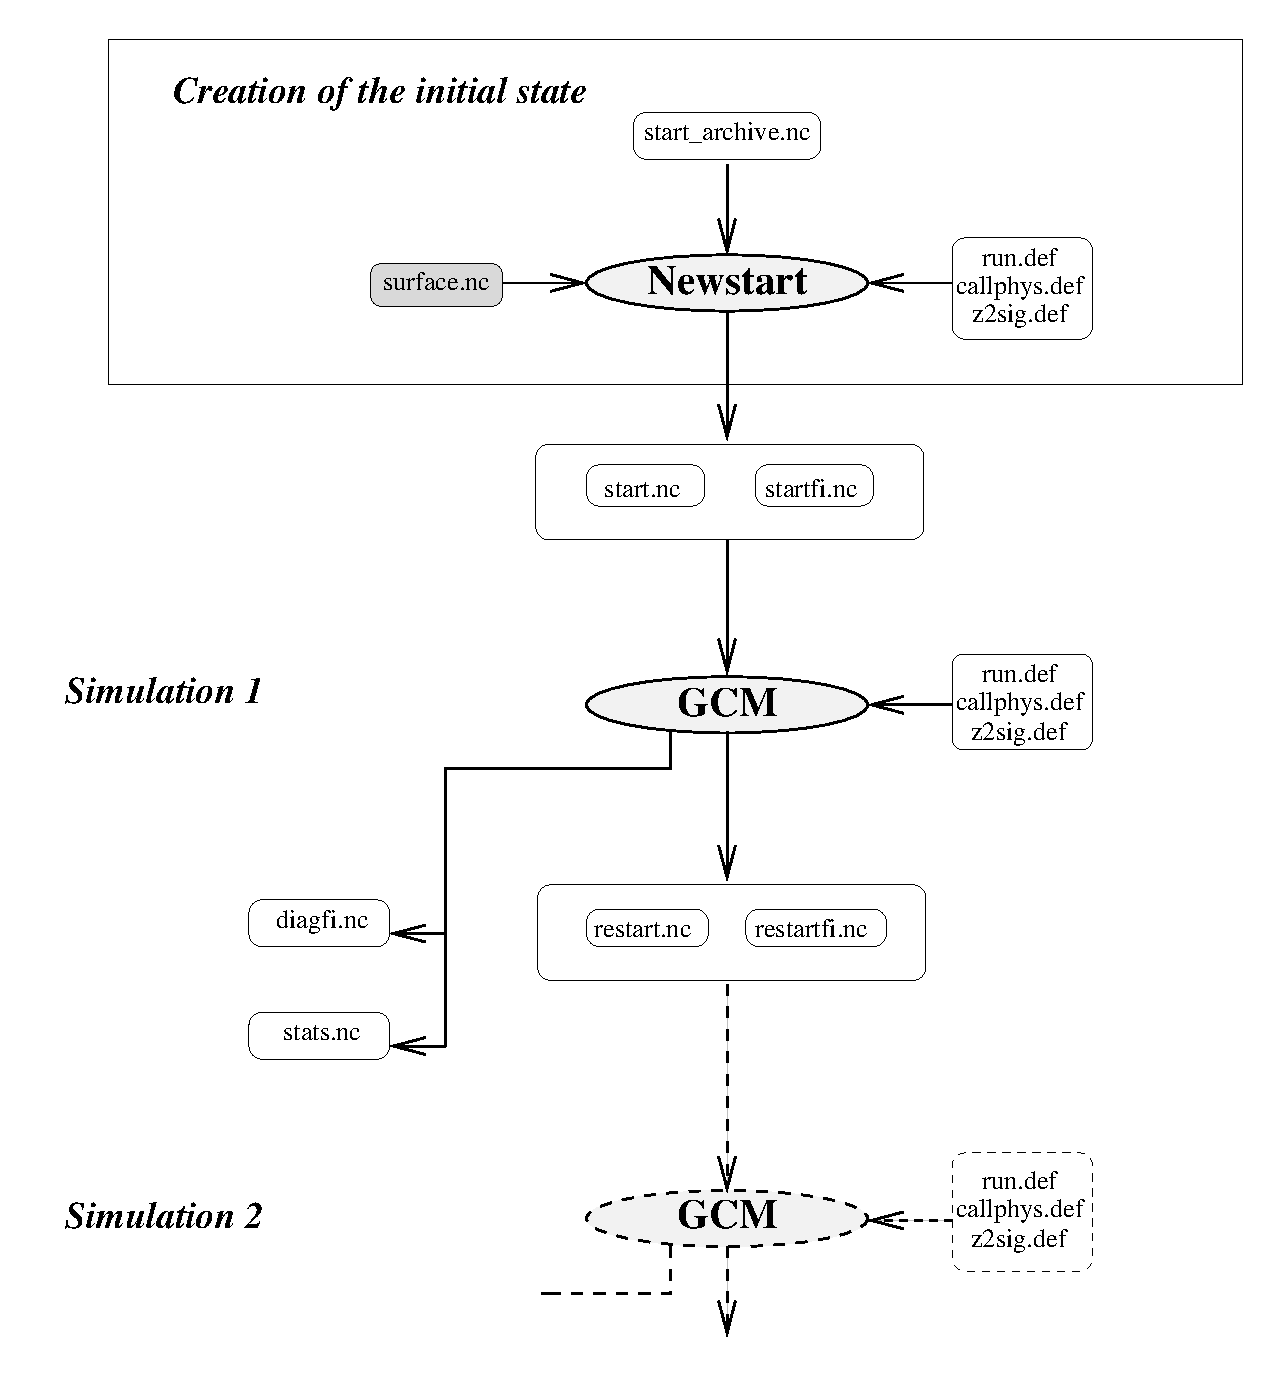
\includegraphics[width=1.2\textwidth]{Fig/inout.eps}}}
\caption{Input/output data}
\label{fig:inout}
\end{figure}

IMPORTANT: The following line MUST be in file run.def (or callphys.def): 
\begin{verbatim}
planet_type = mars
\end{verbatim}
for using LMDZ.MARS model or
\begin{verbatim}
planet_type = generic
\end{verbatim}
for using LMDZ.GENERIC model.

\begin{itemize}
\item[$\bullet$] To run the serial {\bf gcm.e} interactively:\\
Once you have the program {\bf gcm.e},
input files {\bf start.nc} {\bf startfi.nc},
and parameter files {\bf run.def, callphys.def, gases.def, traceur.def, and z2sig.def}
in the same directory, simply execute the program to run a simulation:
\begin{verbatim}
gcm.e
\end{verbatim}

You might need more memory. Use \verb|ulimit -s unlimited| to change user limits.\\
You might also want to keep all messages and diagnostics written to standard
output (i.e. the screen). You should then redirect the standard output
(and error) to some file, e.g. {\tt gcm.out}:\\
If using Csh:
\begin{verbatim}
gcm.e >! gcm.out
\end{verbatim}
If using Bash:
\begin{verbatim}
gcm.e > gcm.out 2>&1
\end{verbatim}


\item [$\bullet$] To run the MPI-parallel {\bf gcm.e} interactively:
\begin{verbatim}
mpirun -np N gcm.e > gcm.out 2>&1
\end{verbatim}
\verb|-np N| specifies the number of procs to run on.\\
IMPORTANT: one MUST use the \verb|mpirun| command corresponding to the \verb|mpif90| compiler specified in the \verb|arch| file.\\
Output files (restart.nc, diagfi.nc ,etc.) are just as when running in serial. But standard output messages are written by each process.\\
If using chained simulations (run\_mcd/run0 scripts), then the command line to run the gcm in \verb|run0| must be adapted for local settings.\\
NB: LMDZ.COMMON dynamics set to run in double precision, so keep \verb|NC_DOUBLE| declaration (and real to double precision promotion) in the arch files.
\item [$\bullet$] To run the hybrid parallel {\bf gcm.e} interactively:
\begin{verbatim}
export OMP_NUM_THREADS=2
export OMP_STACKSIZE=2500MB
mpirun -np 2 gcm.e > gcm.out 2>&1
\end{verbatim}
In this exemple, each of the 2 process MPI have 2 OpenMP tasks with a 2500MB memory.
\item[$\bullet$] To run the MPI-parallel {\bf gcm.e} with a job scheduler (different on each machine):
\begin{verbatim}
PBS example (on Ciclad):
#PBS -S  /bin/bash
#PBS -N  job_mpi08
#PBS -q short
#PBS -j eo
#PBS -l "nodes=1:ppn=8"
# go to directory where the job was launched
cd $PBS_O_WORKDIR
mpirun gcm_64x48x29_phymars_para.e > gcm.out 2>&1
\end{verbatim}
\begin{verbatim}
LoadLeveler example (on Gnome):
# @ job_name = job_mip8
# standard output file  
# @ output = job_mpi8.out.$(jobid)
# standard error file
# @ error =  job_mpi8.err.$(jobid)
# job type
# @ job_type = mpich
# @ blocking = unlimited
# time
# @ class = AP
# Number of procs 
# @ total_tasks = 8
# @ resources=ConsumableCpus(1) ConsumableMemory(2500 mb)
# @ queue
set -vx
mpirun gcm_32x24x11_phymars_para.e > gcm.out 2>&1
\end{verbatim}
\begin{verbatim}
LoadLeveler example (on Ada):
module load intel/2012.0
# @ output  =  output.$(jobid)
# @ error = $(output)
# @ job_type = parallel
## Number of MPI process
# @ total_tasks = 8
## Memory used by each MPI process
# @ as_limit = 2500mb 
# @ wall_clock_limit=01:00:00
# @ core_limit = 0
# @ queue
set -x
poe ./gcm.e -labelio yes > LOG 2>&1
\end{verbatim}
\item[$\bullet$] To run the hybrid MPI/OpenMP-parallel {\bf gcm.e} with a job scheduler (different on each machine):
\begin{verbatim}
LoadLeveler example (on Gnome):
# @ job_name = job_mip8
# standard output file  
# @ output = job_mpi8.out.$(jobid)
# standard error file
# @ error =  job_mpi8.err.$(jobid)
# job type
# @ job_type = mpich
# @ blocking = unlimited
# time
# @ class = AP
# Number of procs 
# @ total_tasks = 8
# @ resources=ConsumableCpus(1) ConsumableMemory(5000 mb)
# @ queue
set -vx
export OMP_NUM_THREADS=2 #sinon par defaut, lance 8 threads OpenMP
export OMP_STACKSIZE=2500MB
mpirun gcm_32x24x11_phymars_para.e > gcm.out 2>&1
\end{verbatim}
IMPORTANT: ConsumableMemory must be equal to OMP\_NUM\_THREADSxOMP\_STACKSIZE.\\
In this case, we are using 8x2 cores.
\begin{verbatim}
LoadLeveler example (on Ada):
module load intel/2012.0
# @ output  =  output.$(jobid)
# @ error = $(output)
# @ job_type = parallel
## Number of MPI process
# @ total_tasks = 8
## Number of OpenMP tasks attached to each MPI process
# @ parallel_threads = 2
## Memory used by each MPI process
# @ as_limit = 5gb 
# @ wall_clock_limit=01:00:00
# @ core_limit = 0
# @ queue
set -x
export OMP_STACKSIZE=2500MB
poe ./gcm.e -labelio yes > LOG 2>&1
\end{verbatim}
IMPORTANT: In this case, each core needs 2.5gb and we are using 2 OpenMP tasks for each MPI process so $\verb|as_limit|=2 \times 2.5$.
\end{itemize}
%**********
\section{Visualizing the output files}

As the model runs it generates output files {\bf diagfi.nc} and
{\bf stats.nc} files. The former contains instantaneous values of
various fields and the later statistics (over the whole run) of some
variables.

\subsection{Using GrAds to visualize outputs}
If you have never used the graphic software {\bf GrAds}, we strongly
recommend spending half an hour to familiarize yourself with it by following
the demonstration provided for that purpose.
The demo is fast and easy to follow and you will learn the basic commands.
To do this read file
\begin{verbatim}
/distrib/local/grads/sample
\end{verbatim}

For example, to visualize files {\tt diagfi.nc} and {\tt stats.nc}

NetCDF files {\tt diagfi.nc} and {\tt stats.nc} can be accessed directly
using GrAdS thanks to utility program gradsnc,
(the user does not need to intervene).\\

\noindent
To visualize the temperature in the 5th layer using file
{\tt diagfi.nc} for example:
\label{loc:visu}

\begin{description}
\item {\bf -} GrAdS session:

  \begin{description}
  \item \verb+grads+ {\it return}

  \item {\it return} (opens a landscape window)

  \item \verb+ga-> sdfopen diagfi.nc+

  \item \verb+ga-> query file+ (displays info about the open file, including the name of the stored variables. Shortcut: {\it q file})

  \item \verb+ga-> set z 5+ (fixes the altitude to the 5th layer)

  \item \verb+ga-> set t 1+ (fixes the time to the first stored value)

  \item \verb+ga-> query dims+ (indicates the fixed values for the 4
  dimensions. Shortcut: {\it q dims})

  \item \verb+ga-> display temp+ (displays the temperature card for the 5th layer and for the first time value stored. Shortcut: {\it d
  T})

  \item \verb+ga-> clear+ (clears the display. Shortcut: {\it c})

  \item \verb+ga-> set gxout shaded+ (not a contour plot, but a shaded one)

  \item \verb+ga-> display temp+

  \item \verb+ga-> set gxout contour+ (returns to contour mode to display the levels)

  \item \verb+ga-> display temp+ (superimposes the contours if the clear command is not used)

  \end{description}
\end{description}



%%%%%%%%%%%%%%%%%%%%%%%%%%%%%%%%%%%%%%%%%%%%%%%%%%%%%%%%%%%%%%%%%%%%%%%

\section{Resuming a simulation}
At the end of a simulation, the model generates {\bf restart} files
(files {\tt restart.nc} and {\tt restartfi.nc})
which contain the final state of the model.
As shown in figure~\ref{fig:inout},
these files (which are of the same format as the start files)
can later be used as initial
states for a new simulation.\\

\noindent
The {\bf restart} files just need to be renamed:
\begin{verbatim}
mv restart.nc start.nc
mv restartfi.nc startfi.nc
\end{verbatim}
\noindent
and running a simulation with these will in fact resume the simulation
from where the previous run ended.

\section{Chain simulations}

In practice, we recommend running a chain of simulations lasting several
days or longer (or hundreds of days at low resolution).

To do this, a script named {\tt run0} is available in
\verb+LMDZ.GENERIC/deftank+ , which should be used as follows:
\begin{itemize}
\item Set the length of each simulation in {\tt run.def}
 (i.e. set the value of {\tt nday})
\item Set the maximum number of simulations at the beginning of the {\tt run0}
script (i.e. set the value of {\tt nummax})
\item Copy start files {\tt start.nc  startfi.nc} over and rename them
      {\tt start0.nc startfi0.nc}.
\item Run script {\tt run0}
\end{itemize}

{\tt run0} runs a series of simulations that generate the indexed output
files (e.g. {\tt start1, startfi1, diagfi1}, etc.)
including files {\tt lrun1, lrun2}, etc. containing the redirection of the
display and the information about the run.

{\it NOTE:} to restart a series of simulations after a first series
(for example, starting from {\tt start5 and  startfi5}), just write the
index of the initial files (e.g. 5) in the file named {\tt num\_run}.
If {\tt num\_run} exists, the model will start from the index written in
{\tt num\_run}. If not it will start from, {\tt start0 and startfi0}.


{\it NOTE}: A script is available for performing annual runs with 12 seasons
at 30$^o$ solar longitude
as it is in the database (script {\bf \tt run\_mcd}, also found in directory
{\tt deftank}).
This script functions with script run0. Just set the number of simulations to
1 in run0. Then copy run.def into run.def.ref and set nday to 9999 in this
file. To start from startN.c, edit the file run\_mcd and comment
(with a \#) the N months already created and describe N in {\tt num\_run}.
Then run  {\bf \tt run\_mcd}.


\section{Creating and modifying initial states}

\label{sc:newstart}

\subsection{Using program ``newstart''}

When working with the generic model, it is common to start with simple initial conditions (e.g., isothermal, motionless atmosphere). For this we create an initial state using {\bf newstart}. In practice, we usually take an old initial state, and simply modify it.

Like the GCM, the program {\bf newstart} must be compiled (using the {\tt makegcm} script) to the required grid resolution.
For example:
\begin{verbatim}
makegcm -d 32x32x20 -p std newstart
\end{verbatim}

Then run

\begin{verbatim}
newstart.e
\end{verbatim}

The program then gives you two options:

\begin{verbatim}
 From which kind of files do you want to create newstart and startfi files
     0 - from a file start_archive
     1 - from files start and startfi
\end{verbatim}

\begin{itemize}
\item{-} Option ``1'' allows you to read and modify the information needed
to create a new initial state  from the files
\verb+ start.nc, startfi.nc +
\item{-} Option ``0'' allows you to read and modify the information needed to
create a new initial state from file
\verb+ start_archive.nc + (whatever the \verb+ start_archive.nc +
grid resolution is).\\
\end{itemize}
If you use tracers, make sure that they are taken into account in your
start files (either start or start\_archive).\\ \\
Then answer to the various questions in the scroll menu.
These questions allow you to modify the initial state for the following
parameters.\\


{\footnotesize
\begin{verbatim}
 First set of questions:
 Change values in tab_cntrl ? :
 ~~~~~~~~~~~~~~~~~~~~~~~~~~~~~~
 (Current values given above)

 (3)          day_ini : Initial day (=0 at Ls=0)
 (19)              z0 :  surface roughness (m)
 (21)       emin_turb :  minimal energy (PBL)
 (20)         lmixmin : mixing length (PBL)
 (26)         emissiv : ground emissivity
 (24 et 25)   emisice : CO2 ice max emissivity
 (22 et 23)  albedice : CO2 ice cap albedos
 (31 et 32) iceradius : mean scat radius of CO2 snow
 (33 et 34) dtemisice : time scale for snow metamorphism
 (27)        tauvis : mean dust vis. reference opacity
 (35)      volcapa : soil volumetric heat capacity
 (18)     obliquit : planet obliquity (deg)
 (17)     peri_day : periastron date (sols since Ls=0)
 (15)     periastr : min. star-planet dist (Mkm)
 (16)     apoastr  : max. star-planet (Mkm)
 (14)     year_day : length of year (in sols)
 (5) rad : radius of the planet (m)
 (6) omeg : planet rotation rate (rad/s)
 (7) g : gravity (m/s2)
 (8) mugaz : molecular mass of the atmosphere (g/mol)
 (9) rcp : r/Cp
 (10) daysec : length of a sol (s)

 Second set of questions :
 flat : no topography ("aquaplanet")
 bilball : uniform albedo and thermal inertia
 coldspole : cold subsurface and high albedo at S.pole
 qname : change tracer name
 q=0 : ALL tracer =zero
 q=x : give a specific uniform value to one tracer
 ini_q : tracers initialisation for chemistry, water and ice
 ini_q-H2O : tracers initialisation for chemistry and ice
 ini_q-iceH2O : tracers initialisation for chemistry only
 noglacier : Remove tropical H2O ice if |lat|<45
 watercapn : H20 ice on permanent N polar cap
 watercaps : H20 ice on permanent S polar cap
 oborealis : H2O ice across Vastitas Borealis
 iceball   : Thick ice layer all over surface
 wetstart  : start with a wet atmosphere
 isotherm  : Isothermal Temperatures, wind set to zero
 radequi   : Earth-like rad. eq. temperature profile and winds set to zero
 co2ice=0 : remove CO2 polar cap
 ptot : change total pressure
 emis : change surface emissivity
 therm_ini_s : Set soil thermal inertia to reference suface values
\end{verbatim}
}


Program {\bf newstart.e} creates files
{\tt restart.nc} and {\tt restartfi.nc}
that you generally need to rename (for instance rename them in start0.nc
and startfi0.nc if you want to use run0 or run\_mcd, starting with season 0;
rename them {\tt start.nc} and {\tt startfi.nc} if you just want to perform
one run with {\tt gcm.e}).


\subsection{Creating the initial start\_archive.nc file }

Archive file
{\tt start\_archive.nc} is created from files
{\tt start.nc} and {\tt startfi.nc} by program {\bf start2archive}.
Program {\bf start2archive} compiles to the same grid resolution as the
{\tt start.nc} and {\tt startfi.nc} grid resolution. For example:

\begin{verbatim}
makegcm -d 32x32x20 -p std start2archive
\end{verbatim}
Then run \verb+ start2archive.e+ \\ \\
You now have a \verb+ start_archive.nc+ file for one season that you can
use with newstart.
If you want to gather other states obtained at other times of year, rerun
{\tt start2archive.e} with the {\tt start.nc} and {\tt startfi.nc}
 corresponding to these.
These additional initial states will automatically be added to the
{\tt start\_archive.nc} file present in the directory.

\subsection{Changing the horizontal or vertical grid resolution}

To run at a different grid resolution than available initial conditions
files, one needs to use tools {\bf newstart} and {\bf start2archive}

For example, to create initial states at grid resolution
32$\times$24$\times$25 from NetCDF files
\verb+ start + and \verb+ startfi + at grid resolution
  64$\times$48$\times$32 :

\begin{itemize}
\item Create file \verb+ start_archive.nc +
with {\bf start2archive.e} compiled at grid resolution
64$\times$48$\times$32 using {\bf old file {\tt z2sig.def}
 used previously}

\item Create files
{\tt newstart.nc} and {\tt newstartfi.nc}
 with {\bf newstart.e}
compiled at grid resolution 32$\times$24$\times$25,
using {\bf new file {\tt z2sig.def}}

\end{itemize}

[NOT RELEVANT??]
If you want to create starts files with tracers for 50 layers using a
{\tt start\_archive.nc} obtained for 32 layers, do not forget to use the
\verb+ ini_q+ option in newstart in order to correctly initialize tracers
value for layer 33 to layer 50.
You just have to answer yes to the question on thermosphere initialization
if you want to initialize the thermosphere part only (l=33 to l=50),
and no if you want to initialize tracers for all layers (l=0 to l=50).\\ \\

